\begin{figure}[h]
\begin{center}
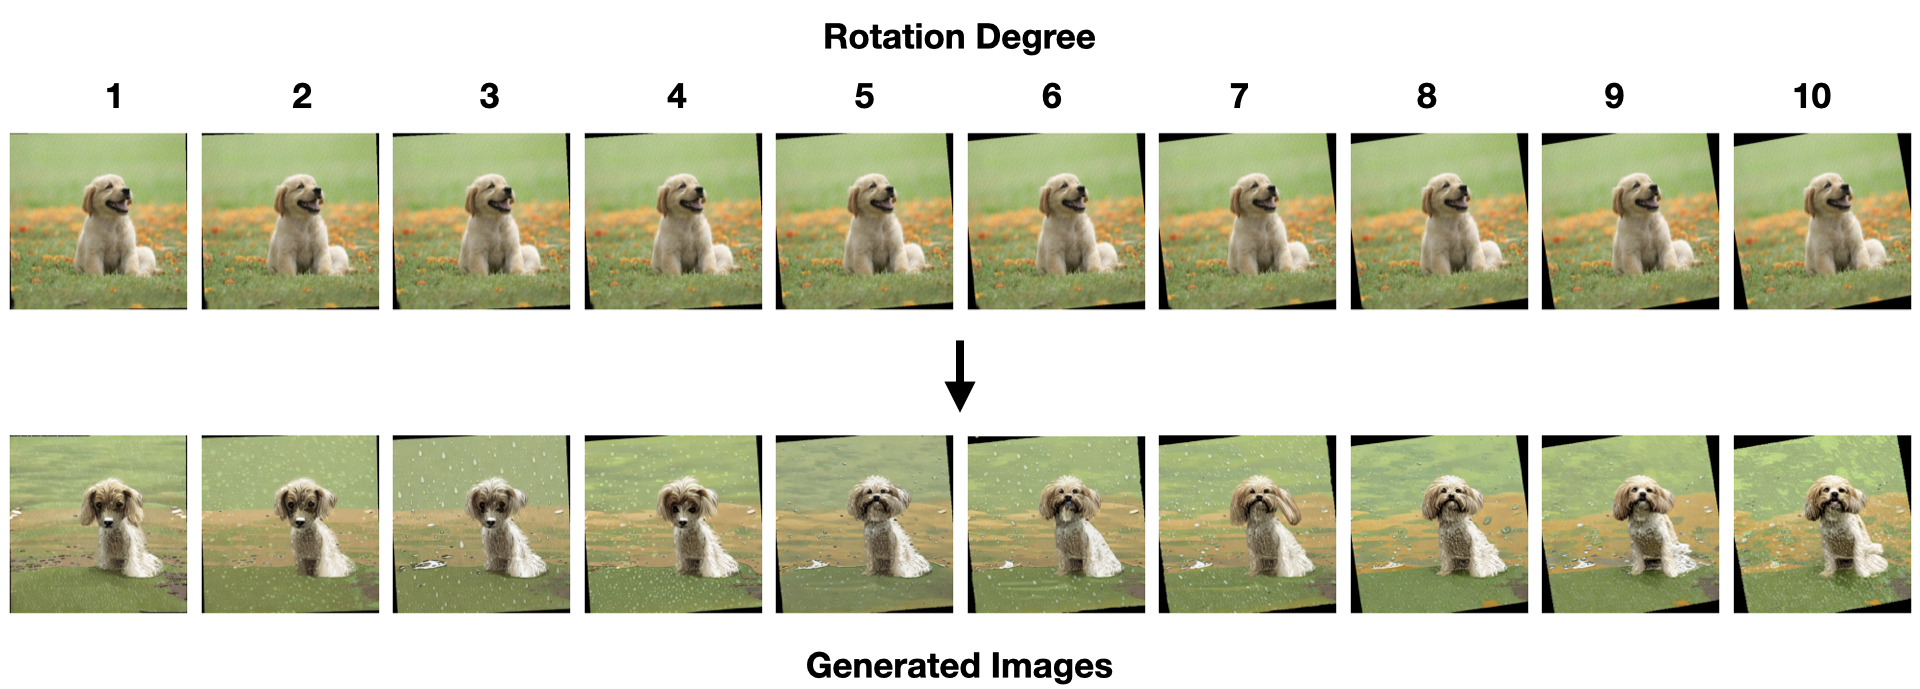
\includegraphics[width=\textwidth]{images/rotation-figure.001.png}
\end{center}
\caption{\textbf{Rotations of photoguard images}. First row: We perform counter-clockwise rotations of varying angles on a photoguard image. Second row: Starting from the rotated image above, the adversary uses a diffusion model to make edits according to the same prompt setup as Figure~\ref{fig:img2img-overview}. The generated image does not retain the original subject in any of the rotations we tried.}
\label{figure-rotation}
\end{figure}